\begin{center}
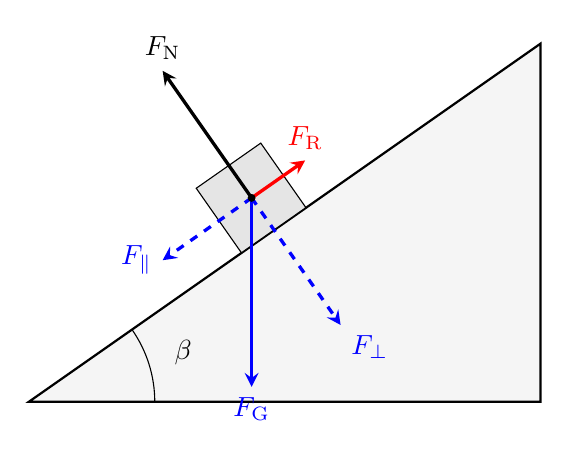
\begin{tikzpicture}[>=stealth]
 \draw[thick, fill=gray!8] (0,0) -- (6.50,0) -- (6.50,4.55) -- cycle;
 \draw (1.6,0) arc (0:35:1.6);
 \node at (1.96,0.62) {$\beta$};
 \begin{scope}[shift={(3.11,2.18)}, rotate=35]
  \draw[fill=gray!20] (-0.5,0) rectangle (0.5,1.0);
 \end{scope}
 \draw[->, very thick, blue] (2.83,2.59) -- ++(-90.00:2.40) node[anchor=north] {$F_\mathrm{G}$};
 \draw[->, very thick, blue, dashed] (2.83,2.59) -- ++(-55.00:1.97) node[anchor=north west] {$F_\perp$};
 \draw[->, very thick, blue, dashed] (2.83,2.59) -- ++(215.00:1.38) node[anchor=east] {$F_\parallel$};
 \draw[->, very thick, black] (2.83,2.59) -- ++(125.00:1.97) node[anchor=south] {$F_\mathrm{N}$};
 \draw[->, very thick, red] (2.83,2.59) -- ++(35.00:0.83) node[anchor=south] {$F_\mathrm{R}$};
 \fill (2.83,2.59) circle (0.05);
\end{tikzpicture}
\end{center}

Auf den gleitenden Würfel wirken entlang der Ebene die Hangabtriebskraft $m\,g\sin\alpha$ und die Gleitreibungskraft $\mu_\mathrm{G}\,F_\mathrm{N} = \mu_\mathrm{G}\,m\,g\cos\alpha$. Für Stahl auf Stahl ist $\mu_\mathrm{G} = \muGO$ (FoTaBe S.~189).

Gleichförmig gleitet er, wenn sich die beiden Kräfte aufheben: $m\,g\sin\alpha = \mu_\mathrm{G}\,m\,g\cos\alpha$, also $\tan\alpha = \mu_\mathrm{G}$ und
\begin{align}
 \alpha &= \wiF = \arctan\left(\muG\right) = \wi \approx \result{\wiP{0}{2}}
\end{align}

Bei $\beta = \wiBO$ ist die Hangabtriebskraft grösser als die Reibungskraft. Das Aktionsprinzip $m\,a = m\,g\sin\beta - \mu_\mathrm{G}\,m\,g\cos\beta$ gibt
\begin{align}
 a &= \aWuF \\
   &= \gE\cdot\left(\sin\left(\wiBO\right)-\muG\cdot\cos\left(\wiBO\right)\right) \\
   &= \aWu \approx \result{\aWuP{0}{2}}
\end{align}
Diese Beschleunigung gilt, sobald der Würfel gleitet. Aus der Ruhe setzt er sich bei \wiBO\ noch nicht von selbst in Bewegung: Mit der Haftreibungszahl $\mu_\mathrm{H} = \muHO$ beginnt er erst ab $\wiHP{0}{2}$ zu rutschen; man muss ihn also anstossen.
